\documentclass[twocolumn]{phdsymp}

\usepackage[english]{babel}
\usepackage[T1]{fontenc}
\usepackage[utf8]{inputenc}

\usepackage{amsmath, amsfonts, amssymb}
\usepackage{ctable} % Usage: \ctable[options]{column def like c|c|r|l}{\tnote commands for footnotes}{normal table content}, with \tnote[symbol]{text} footnote definitions, and \tmark[symbol] used to reference the footnote in the normal table content
\usepackage{graphicx} % Figures
\usepackage{hyperref} % Creates links (boxes in various colors around words)
\usepackage[capitalise]{cleveref} % LOAD AFTER HYPERREF!!!
\usepackage{times}
\usepackage[super]{nth} % 2nd with nd in superscript
\usepackage{siunitx}
\usepackage{physics} % Vector calculus etc.
% \usepackage{subcaption} % Enables subfigures


\setlength{\paperheight}{11in} % Package hyperref
\def\BibTeX{{\rm B\kern-.05em{\sc i\kern-.025em b}\kern-.08em
    T\kern-.1667em\lower.7ex\hbox{E}\kern-.125emX}}

%%%% PACKAGES SETUP COMMANDS
\hypersetup{colorlinks=true,
    urlcolor=black,
    citecolor=gray}

% MuMax3
\newcommand{\mumax}{$\mathsf{mumax}^3$}
% Mono-spaced inline code (for multiline code, use package 'listings')
\newcommand{\code}[1]{\texttt{#1}}
% Numbers a single line in a no-numbering multiline equation* or align*
\newcommand{\numberthis}{\addtocounter{equation}{1}\tag{\theequation}}
% Vertical line between subplots
\newcommand{\rulesep}{\unskip\ \vrule\ }


\begin{document}

\title{Biaxial nanomagnets as building block for balanced half-adders}

\author{Jonathan Maes \thanks{J.~Maes is a student in the \nth{2} year of the Master of Science in Engineering Physics (2020-2021), Ghent University (UGent), Ghent, Belgium. E-mail: \href{mailto:Jonathan.Maes@UGent.be}{Jonathan.Maes@UGent.be}.}}

\supervisor{Bartel Van Waeyernberghe, Jonathan Leliaert, Pieter Gypens}

\maketitle

\begin{abstract}
Nanomagnetic logic implements logic gates by making use of magnetostatic interactions between closely spaced single-domain nanomagnets. A biaxial nanomagnet has four stable magnetization directions, and can therefore represent two bits of information. Since a half adder takes two bits as input and yields two bits as output, a half adder can naturally be implemented using biaxial nanomagnets. Since each nanomagnet influences every other nanomagnet, and vice versa, there exists a two-way flow of information between in- and output. This allows for reverse calculations, but only if the ground states of all possible inputs have equal energy, in which case the gate is termed `balanced'. Here, a geometry is proposed which can function as a half adder in a forward calculation, consisting of two free biaxial islands aligned along their easy axes, and one fixed island to break the symmetry and realize the correct logical behavior.  % TODO: expand
\end{abstract}

\begin{keywords}
biaxial nanomagnets, nanomagnetic logic, half adder, balanced logic gates
\end{keywords}

\section{Introduction}
\PARstart{I}{n} a ferromagnetic material, the magnetic moments of neighboring atoms prefer a parallel alignment. As such, a lithographically etched ferromagnetic island of small size, on the order of a hundred nanometers, will have a nearly uniform magnetization, close to saturation~\cite{NML_Carlton,MQCA_RoomTemp}, but with small deviations from this uniformity to accommodate for the geometry of the island. By choosing a geometry with four-fold rotational symmetry, the island can be made to exhibit biaxial shape anisotropy, hence creating two stable axes, such that the magnetization prefers to point along any of four in-plane directions. These can be used to represent exactly two bits of information. As such, these nanomagnetic islands can be used to create a digital logic circuit. This is called nanomagnetic logic (NML), a computing architecture which propagates binary information through dipolar field coupling between the magnetization of closely spaced nanomagnets~\cite{SubnanosecondPropagation_AnisotropyChains}, and is promising for its extremely low energy dissipation per operation~\cite{SubnanosecondPropagation_AnisotropyChains,FourStateLogic,MQCA_RoomTemp}. NML can be used to perform forward logic operations, which propagate information from an input to an output, much like traditional digital logic technologies. Such traditional architectures, however, use field-effect transistors to control the flow of electrons, which only allows information to flow in one direction. In NML, all islands influence each other, such that there is fundamentally a two-way flow of information, thus allowing a fundamentally different way of thinking about logic. This is provided by `terminal-agnostic' logic~\cite{FactorizationMemcomputing}, which can give NML an edge over traditional CMOS technology. Such a terminal-agnostic gate is able to self-organize into its logically correct states, such that it does not matter whether the information is fed at what would traditionally be considered the input or output. To achieve this using NML, one has to make use of `balanced' gates. These are gates for which the ground states corresponding to all possible inputs have equal energy~\cite{GYP-18}. A necessary condition for a gate to be balanced, is that the number of distinguished configurations with minimum energy is equal to the number of input combinations the automaton handles~\cite{QCA_Algorithms}. If this condition is fulfilled, all logically correct states will have an equal probability of occurring at nonzero temperatures. Conversely, when applying the desired output, all the correct inputs which should yield that output will be equally likely to occur, thus allowing reversible logic operations. There have been examples in literature where majority logic gates and balanced NAND gates have been created using uniaxial nanomagnets~\cite{GYP-18}. \par
By using biaxial nanomagnets, smaller logic gates can be created due to the increased integration density as compared to uniaxial islands. The goal here, is to realize a nanomagnetic half adder. Because a half adder takes two input bits and yields two output bits, it feels almost natural to use biaxial nanomagnets for this purpose.
% TODO: talk about tendency to align along long axis

%% NOTE: "\itemindent -1em \leftmargini 2em" . Sometimes other values
%% are used, e.g. "\itemindent 2em \leftmargini 0em"
\begin{itemize}
\item Introduction: QCA, signal propagation uniaxial and biaxial
\item Physics: thermal fluctuations
\item Biaxial island: optimal external field magnitude short explanation, higher order energy barrier mention without figure, numerical error short explanation, thermal switching f0 conclusions
\item Half adder:  sum up some considerations, then sweep s and d far from common axis and discuss different conventions shortly, then balancedness is bad, then show energy levels and multiple gates in series, then sweep s and d close to common axis and say balancedness is better but not optimal, show energy levels too
\item \ldots{}
\end{itemize}

\section{Theoretical framework}
A theoretical framework suitable for investigating nanomagnetic logic is provided by the micromagnetic theory. In this formalism, instead of considering all individual magnetic moments, the magnetization is represented by the continuous magnetization field, denoted by $\vb{M}(\vb{r})=M_{\mathrm{sat}} \vb{m}(\vb{r})$, which has constant norm. This continuum approximation is only applicable locally in ferromagnets, over scales smaller than the exchange length $\lambda$. The time evolution of this theory is described by the Landau-Lifshitz equation~\cite{lifdau}. This theory can be discretized and solved using a finite difference approach, with cell sizes on the order of $\lambda$. This allows efficient calculation of nanomagnetic problems, and several numerical solvers are available for this purpose. Here, the GPU-accelerated \mumax{} software is used~\cite{MuMax3}. It calculates the space-and time-dependent magnetization dynamics in nano- to macro-sized ferromagnets, which is well suited for the problems considered here.

\section{Biaxial island}
Before considering half adders, we must first examine the characteristics of the biaxial nanomagnets themselves. The energy barrier is one of the main factors influencing the thermal switching between stable states. This energy barrier is mainly determined by the shape of the island. Here, we consider the geometry shown in \cref{fig:EA_geom}, which is the union of two identical perpendicular ellipses, and was chosen because it should be reasonably easy to manufacture due to the lack of sharp corners. \par
This geometry is uniquely defined by the length of the long and short axes of the ellipse. The \textit{roundness} $\rho$ is defined as the ratio of the short over the long axis, and the overall \textit{size} $L$ as the length of the long axis. For example, the geometry in \cref{fig:EA_geom} corresponds to $(\rho,L) = (0.55, \SI{100}{\nano\metre})$. The angle \SI{0}{\degree} is defined as the direction pointing to the right, with positive angles in the anticlockwise direction. \par
\begin{figure}
    \centering
    \includegraphics[width=0.4\columnwidth]{Figures/geomPlus55.png}
    \caption{Typical geometry of the biaxial island, the union of two perpendicular ellipses.}
    \label{fig:EA_geom}
\end{figure}
Furthermore, the in-plane angles of several quantities will be used: $\Theta$ denotes the instantaneous average magnetization angle, and its tilde counterpart $\widetilde{\Theta}$ the angle of the magnetization when it is relaxed to a local energy minimum. The angle of an external bias field is denoted by $\chi$, while its tilde counterpart $\widetilde{\chi}$ indicates a probing field. This probing field is used in the simulations to prevent the magnetization from fully relaxing to the easy axes, when quantities have to be calculated for situations where the magnetization is not in an anisotropic energy minimum. Finally, $\Phi$ denotes the angle by which the geometry of a biaxial island was rotated, i.e. the angle between its ellipse axes and the numerical Cartesian grid of the simulation domain. \par % TODO: remove the quantities that do not appear in the extended abstract
Before investigating thermal switching, the energy barrier of this geometry must be known.

\subsection{Energy barrier}
All of $E(\widetilde{\Theta}~=~n\SI{45}{\degree}), n\in\mathbb{Z}$ are equilibria, due to the symmetry of the geometry. Of these, 4 are energy minima and 4 are maxima. To determine the energy barrier between stable states, the energy landscape must be known. To accurately calculate the energy landscape, one has to allow the magnetization to settle itself to the geometry. To get the energy at angles which do not correspond to an energy minimum, a probing field is used to keep the magnetization away from this minimum. The Zeeman energy term due to this probing field is then subtracted, to reveal the energy landscape of a single biaxial island. This energy landscape is shown in \cref{fig:EA_EnergyLandscape}, for $\rho=0.65$. \par
The height of this energy landscape for the lowest field magnitudes is then the \textit{energy barrier}. It strongly depends on the roundness, as shown in \cref{fig:EA_EnergyRoundnessDependence}. It is observed that, for large $\rho$, the easy axes are the long axes of the ellipses, while the hard axes are the diagonals in between them. For $\rho < 0.48$, the opposite is true. This is understood by looking at the detailed magnetization profile for both large and small $\rho$.

Talk about the barrier(rho) dependence first, and later on talk about the relaxation condition and the different external fields
Smol introduction on the energy barrier, but dont go deep into the probing field, that is better left to the main text. Perhaps talk about the optimal probing field magnitude, but not in much detail. Just say the most important things that are observed for it.
Say stuff about the energy landscape and the dependence on rho, which is quite interesting thing. Also relaxed magnetization profile, but dont show the unstable ones cuz that is gonna take up too much space
Then talk about the thermal switching and a bit of the theory behind it, with the arrhenius law for f0 etc. Certainly show the table with simulated values.
\begin{figure}
    \centering
    \includegraphics[width=0.9\columnwidth]{Figures/Plus_65_B25-0.001-div4_a128Pi_plotOptimized.pdf}
    \caption{Energy landscape for various probing field magnitudes, as listed in the legend. The probing field angle $\widetilde{\chi}$ is varied uniformly in 64 steps from \SI{0}{\degree} to \SI{90}{\degree}, for each magnitude, each dot corresponding to one such angle. The horizontal axis denotes the average magnetization angle $\widetilde{\Theta}$ after relaxation, which is not necessarily equal to $\widetilde{\chi}$, especially for low field magnitudes.}
    \label{fig:EA_EnergyLandscape}
\end{figure}
\begin{figure}
    \centering
    \includegraphics[width=0.9\columnwidth]{Figures/Plus_32,64,128_0.1-1_aPi128_B0.01_cell1nm.pdf}
    \caption{Energy barrier as a function of roundness $\rho$, for different total sizes $L$ as listed in the legend. Cell size \SI{1}{\nano\metre}. A positive value indicates that $E(\Theta=\SI{45}{\degree}) > E(\Theta=\SI{0}{\degree})$, i.e. the hard axes are diagonal, while for a negative value the opposite is true.}
    \label{fig:EA_EnergyRoundnessDependence}
\end{figure}

\begin{figure}
     \centering
     \hskip2em
         \includegraphics[width=0.3\columnwidth]{Figures/biaxial_island/BarrierMagnetization/mPlus_roundness0.20_a0.79.png}
     \hskip2em
         \includegraphics[width=0.3\columnwidth]{Figures/biaxial_island/BarrierMagnetization/mPlus_roundness0.60_a0.00.png}
    \caption{Relaxed magnetization for two different geometries with $L=\SI{100}{\nano\metre}$. The color hue represents the in-plane magnetization angle. \textbf{Right:} $\rho=0.2$. \textbf{Left:} $\rho=0.6$.}
    \label{fig:EA_EnergyMagnetization}
\end{figure}


\section{Half adder}
A half adder is a logic gate which adds two binary input bits, and therefore yields two bits as
output. The truth table of a binary half adder is given in the left half of \cref{tab:HalfAdder}. Since both input and output are represented by two bits, they can also each be represented by a biaxial island, because a single biaxial island has 4 stable states and can thus represent exactly two bits of information. As such, a half adder realized with biaxial nanomagnets only has one input island and one output island. The truth table of a half adder represented in the quaternary numeral system inherent to biaxial nanomagnets is given in the right half of \cref{tab:HalfAdder}.
\ctable[
    cap = Half Adder,
    caption = {Truth table for a half adder, both in binary and quaternary numeral systems.},
    label = {tab:HalfAdder},
    pos = ht,
    mincapwidth = 0.7\columnwidth
    ]{
    c|c||c|c % paps vindt dit beter
    }{}{
        \multicolumn{2}{c||}{Binary} & \multicolumn{2}{c}{Quaternary} \\
        \hline
        Input & Output & Input & Output \\
        \hline
        00 & 00 & 0 & 0 \\
        01 & 01 & 1 & 1 \\
        10 & 01 & 2 & 1 \\
        11 & 10 & 3 & 2 \\
    }
\subsection{Nanomagnetic half adders}
When designing a nanomagnetic logic gate, one has to define the meaning of each stable magnetization direction. For biaxial nanomagnets, there are four such directions, which have to be assigned a number from 0 to 3. There are 24 possible ways to do this. We will refer to such a choice as the `\textit{quaternary convention}'. We will always list the quaternary convention in the form $(\SI{0}{\degree}, \SI{90}{\degree}, \SI{180}{\degree}, \SI{270}{\degree})$, for the island geometry from \cref{fig:EA_geom}. A given geometry of nanomagnets, with given input and output islands, will only behave as a half adder for at most one quaternary convention. When choosing a different input or output island, the relevant quaternary convention may be different, or even nonexistent. Thus, given a geometry with $N$ free islands, i.e. whose magnetization direction is not fixed by e.g. the exchange bias, there are $N$ choices for the input island, $N-1$ for the output, and for each such choice there are 24 possible quaternary conventions if one uses the same convention for input and output. Only a select few, if any, of these $24N(N-1)$ possibilities will correctly give the geometry the meaning of a half adder. \par
A given geometry can work as a half adder in a forward calculation if there exists a choice of input island, output island, and quaternary convention, for which the lowest energy state for each of the 4 possible input magnetization angles has the logically correct output magnetization angle. \par
Also note that in any NML system it is necessary to include at least one island whose magnetization direction is permanently fixed, to break the symmetry, since a nanomagnetic system is invariant under a global magnetization reversal~\cite{GYP-18}. Such fixation can for example be realized using the exchange bias.

\subsection{Gate design}
A schematic representation of the half adder proposed here is shown in \cref{fig:EA_HalfAdderConcept1}, where the ground states for all four possible input magnetization directions are shown. The island with the open arrowhead is permanently fixed. The reasoning behind this geometry is as follows. \par
From the truth table of the half adder, it can be noted that there must be two inputs for which input and output are equal: $0\rightarrow0$ and $1\rightarrow1$. This condition is readily fulfilled for two biaxial islands aligned along their easy axes in a `++' geometry. The lowest energy state of such a geometry has both islands with a parallel magnetization along their common axis ($\rightarrow \rightarrow$ or $\leftarrow \leftarrow$). The anti-parallel configuration perpendicular to the common axis ($\uparrow~\downarrow$ or $\downarrow~\uparrow$) is another equilibrium with slightly higher energy, and is stable if the islands have a nonzero energy barrier. \par
As such, two of the four inputs are already mapped to a correct output, if one identifies the horizontal directions with $0$ and $1$ in the quaternary convention. Also $3\rightarrow2$ is fulfilled, as this corresponds to the anti-parallel configuration if one identifies the vertical directions with $2$ and $3$. The only combination which is not yet fulfilled is $2\rightarrow1$, as this then requires a vertical input to be mapped to a horizontal output. This can be fulfilled by adding a permanently fixed island, in the manner shown in \cref{fig:EA_HalfAdderConcept1}. It was already established that the quaternary number 1 corresponds to a horizontal magnetization. Hence, if one identifies the `up' direction with the quaternary number 2, one has to make sure the output is horizontal, and not `down'. This can be done by placing the fixed island such that its magnetization points towards the output island, such that a magnetization in the direction of the fixed island becomes unfavorable for this output island.

\begin{figure*}
\centering
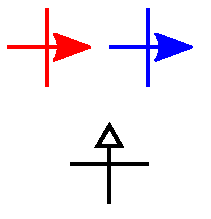
\includegraphics[width=0.15\textwidth]{Figures/HalfAdderConcept/Input 0 deg.pdf}
\rulesep
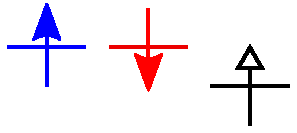
\includegraphics[width=0.15\textwidth]{Figures/HalfAdderConcept/Input 90 deg.pdf}
\rulesep
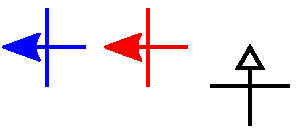
\includegraphics[width=0.15\textwidth]{Figures/HalfAdderConcept/Input 180 deg.pdf}
\rulesep
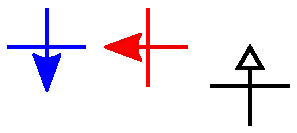
\includegraphics[width=0.15\textwidth]{Figures/HalfAdderConcept/Input 270 deg.pdf}
\caption{Lowest energy configurations for all four possible input magnetizations. This functions as a half adder with quaternary convention $(0,2,1,3)$. Islands with a filled arrowhead can move their magnetization freely to achieve the lowest energy. Islands with an open arrowhead have their magnetization permanently fixed in the direction of the arrow. The blue island is the input island, the red island functions as the output.}
\label{fig:EA_HalfAdderConcept1}
\end{figure*}


\section{Conclusion}
Before considering half adders, the energy landscape of a single biaxial island was examined. It was found that relaxation is necessary for anisotropy to occur; if the island has a perfectly uniform in-plane magnetization, the energy is equal for any of these magnetization directions. The energy barrier significantly depends on the roundness $\rho$ of the ellipses constituting the biaxial island. For large $\rho$, the easy axes are equal to the long axes of these ellipses, with the hard axes diagonally in between these easy axes. For small $\rho$, the easy and hard axes appear to be swapped. This is because the geometry resembles a `plus'-shape, such that each arm of this shape has its own preferred direction. The combination of such vertical and horizontal directions is on average diagonal, with a domain wall in between. For this reason, one must take care when using a biaxial island with low roundness, as the magnetization in the different lobes can differ significantly. At $\rho \approx 0.49$, the energy difference between an average magnetization of \SI{0}{\degree} and \SI{45}{\degree} becomes zero. At this $\rho$, however, the energy landscape is not entirely flat; due to the relaxation of the magnetization along the edges of the geometry, there are 8 stable states instead of 4. \par
The thermal switching of different biaxial islands and for different temperatures and damping constants was also examined. No agreement between theoretical and simulated values for the attempt frequency $f_0$ was found. It was hypothesized that this is because the magnetization of the islands is not perfectly uniform, which is one of the assumptions underlying the theory. The theoretically obtained value $f_0=\SI{6e5}{\per\second}$ is very small compared to the switching frequency, indicating that the theoretical equations are not applicable here. The value obtained through simulations is approximately $f_0=\SI{e10}{\per\second}$,  which is the same order of magnitude as the intrinsic resonance frequency of the magnetization in the local minima of the energy landscape. \par
It was mentioned that biaxial nanomagnets, aligned with their easy axes in an `$\cross \cross$' pattern, can function as a balanced biaxial chain, due to the high degree of symmetry. It is also possible to separately extract the two bits encoded by a single biaxial island, for the $(0,1,3,2)$ quaternary convention. This is done by placing two uniaxial chains along the hard axes. \par
Two similar half adder geometries were proposed, which can perform a forward calculation. One of these geometries has the fixed island far from the common axis, while for the second geometry the fixed island was placed near the common axis. The second has all ground state energies below any of the first excited states, which ensures a correct functioning for a single reverse calculation under ideal circumstances. Unfortunately, in order to chain multiple gates together for a larger reverse calculation, all the ground state energies must be equal, i.e. the gate must be perfectly balanced, which is not the case. \par
The first geometry can not function in reverse at all, as it has excited states with lower energy than some ground states. This geometry does, however, have more spacing in between its energy levels, such that it is better suited for forward calculation. It also has the advantage that it should be relatively straightforward to add some nanomagnetic chains to the input and output, as the fixed island is placed far away from their common axis. \par
%Unfortunately, any half adder following the same concept of using two in-line biaxial islands will never have the ideal quaternary convention $(0,1,3,2)$, because a central part of the reasoning behind this concept requires 0 and 1 to have opposite direction. To resolve these various issues, a radically different geometry will have to be conceived. \par
%The topic of future work can be the continuation of a search for a balanced half adder. A completely new geometry should be designed which is inherently more symmetrical. The asymmetry in the quaternary truth table might prevent a truly mathematically balanced half adder. Including more islands can increase the degrees of freedom, such that a balanced half adder can be approximated by varying geometrical and material parameters.


\section*{Acknowledgments}
The authors would like to acknowledge the suggestions of many people.

% TODO: check if the references are decently formatted, because this bibliography style shows a lot more

\nocite{*}
\bibliographystyle{phdsymp}
\bibliography{smallbibliography}

\end{document}
